% !TEX root = BachelorBookletMain.tex

\chapter{Neural Network Systems}\label{NeuralNetworkSystems}
\section{Data generation}\label{DataGeneration}
The first step is to place markers in the environment where observations should be taken. These markers are scaled Unity cubes where the volume denotes all the valid observation positions, while allowed camera rotations are set in the capturing script. It is possible to group markers and link groups with objects in the environment. Linked objects are then only visible to the capturing camera if the camera is placed in a marker that is in the group the object is linked to.

During data generation, a script moves the camera to a random position and rotation. The camera is then programmatically rendered to a texture and then saved to a file. Camera positioning and capturing can be done multiple times per frame to speed up the generation process. When the file is saved, the position and rotation where the image was taken is saved in the filename of the image. Depending on in which unity scene the image was captured and at what resolution it was set it is sorted automatically into a corresponding folder structure that is created on the fly.

The data generation process can easily be customized in the inspector of the capturing script. In a list, entries can be added that define a capturing resolution and the number of data points to be captured at that resolution. Once the application is run in capturing mode, all data points specified in this list are sequentially generated. On completion a notification sound is played and the environment is automatically shut down.

In the Maze game all structural objects are cubes, where a raised cube represents a wall. This makes it easy to find all valid player positions and generate the markers for the environment automatically.


\section{Model}
To create the neural network model used in this project the Kears functional API is used. Keras is the official front end to Tensorflow and simplifies the creation of neural networks. With the functional API predefined callable class instances, which represent layers, can be used to define a models architecture. For this a class of a layer type is set up and called with the input to the layer. This then returns the output\footnote{The Keras classes don't execute statements immediately, but construct a computation graph for later execution. The output by the layer can be thought of as a pointer that is resolved later, when the model is executed.} of the layer. The outputs can now be feed into another layer. After the model has been described in this manner, Keras can receive optimization parameters e.g. the loss function and then compile the computation graph.

The model created corresponds to the model described in \cref{BackgroundGQN}, with the exception that no latent variables $z$ are used. As encoder and decoder dense networks are used.


\subsection{Saving and loading of network}
To make it easier to identify and reuse models a simple versioning system has been developed. If no specific model is specified to be used, a new one of the specified architecture is created. The model is then given a unique file name consisting of the following: date; time; observation environment; name-ID; version; numeric-ID.

If a request is received to load a specific model, an automatic search is performed for the newest model of the requested id. If a model is found that is newer than the one specified that model is automatically loaded instead of the old one. The versioning of a model is set up so that it increments the version based on the version of the model that is currently being trained.

Keras is used to automatically save the model during training in intervals, preventing total data loss in case of a critical system failure.


\subsection{Data Preprocessing}
First the data is loaded from from disk. Then the data points are normalized. This means that we make all inputs of the data have a range between zero and one. This is required for the used architecture to enable efficient training. The next step is to create a pairings of input data and output labels. This is simply done by choosing all the inputs and outputs from the same environment. These pairings constitute the training data for the model. The output of the model is just a vector, so that we need to rearrange it into a tensor of the original image dimensions. Then we can encode the tensor into a JPEG image.


\section[IPC]{Inter process communication}
Because Python runs outside the Unity environment we need a way to send the network output to Unity. This is done by using a local UDP socket to send the JPEG images to a listening UDP socket in Unity. Because UDP is a connectionless protocol and doesn't give any guaranties that the send data will be received it is a very fast way to send the data. The chance of data getting lost on a local server is very slim and because we are sending a continuous stream we don't care if an image is lost, because we will receive a new one in a few milliseconds.


\section{Rendering}\label{rendering}
Now the data received by the Unity UDP socket gets loaded into a texture. This texture is then rendered to screen. Because our simplified model is unable to render nonstatic objects we need to merge the network output with rendered output from a Unity camera, if we want to use such objects. For this we change the material of objects, we don't want to see in the merged output, to an unlit material of a specific color, referred from here on as the key-out color. This can automatically be done when Unity enters play mode using a script that filters objects based on their layer. \Cref{KeyoutEditor} shows the application of the material form the editor perspective.

Now we render a Unity camera and bit blit the image into a texture using a custom shader that sets all pixels of that are equal to the key-out color to be transparent. Then we apply a pixelation shader to the image to reduce it to the same resolution as the network output. Finally we blit the pixelated version onto the screen over the network rendered output (\cref{RenderMerge}).

\begin{figure}[p]
  \centering
  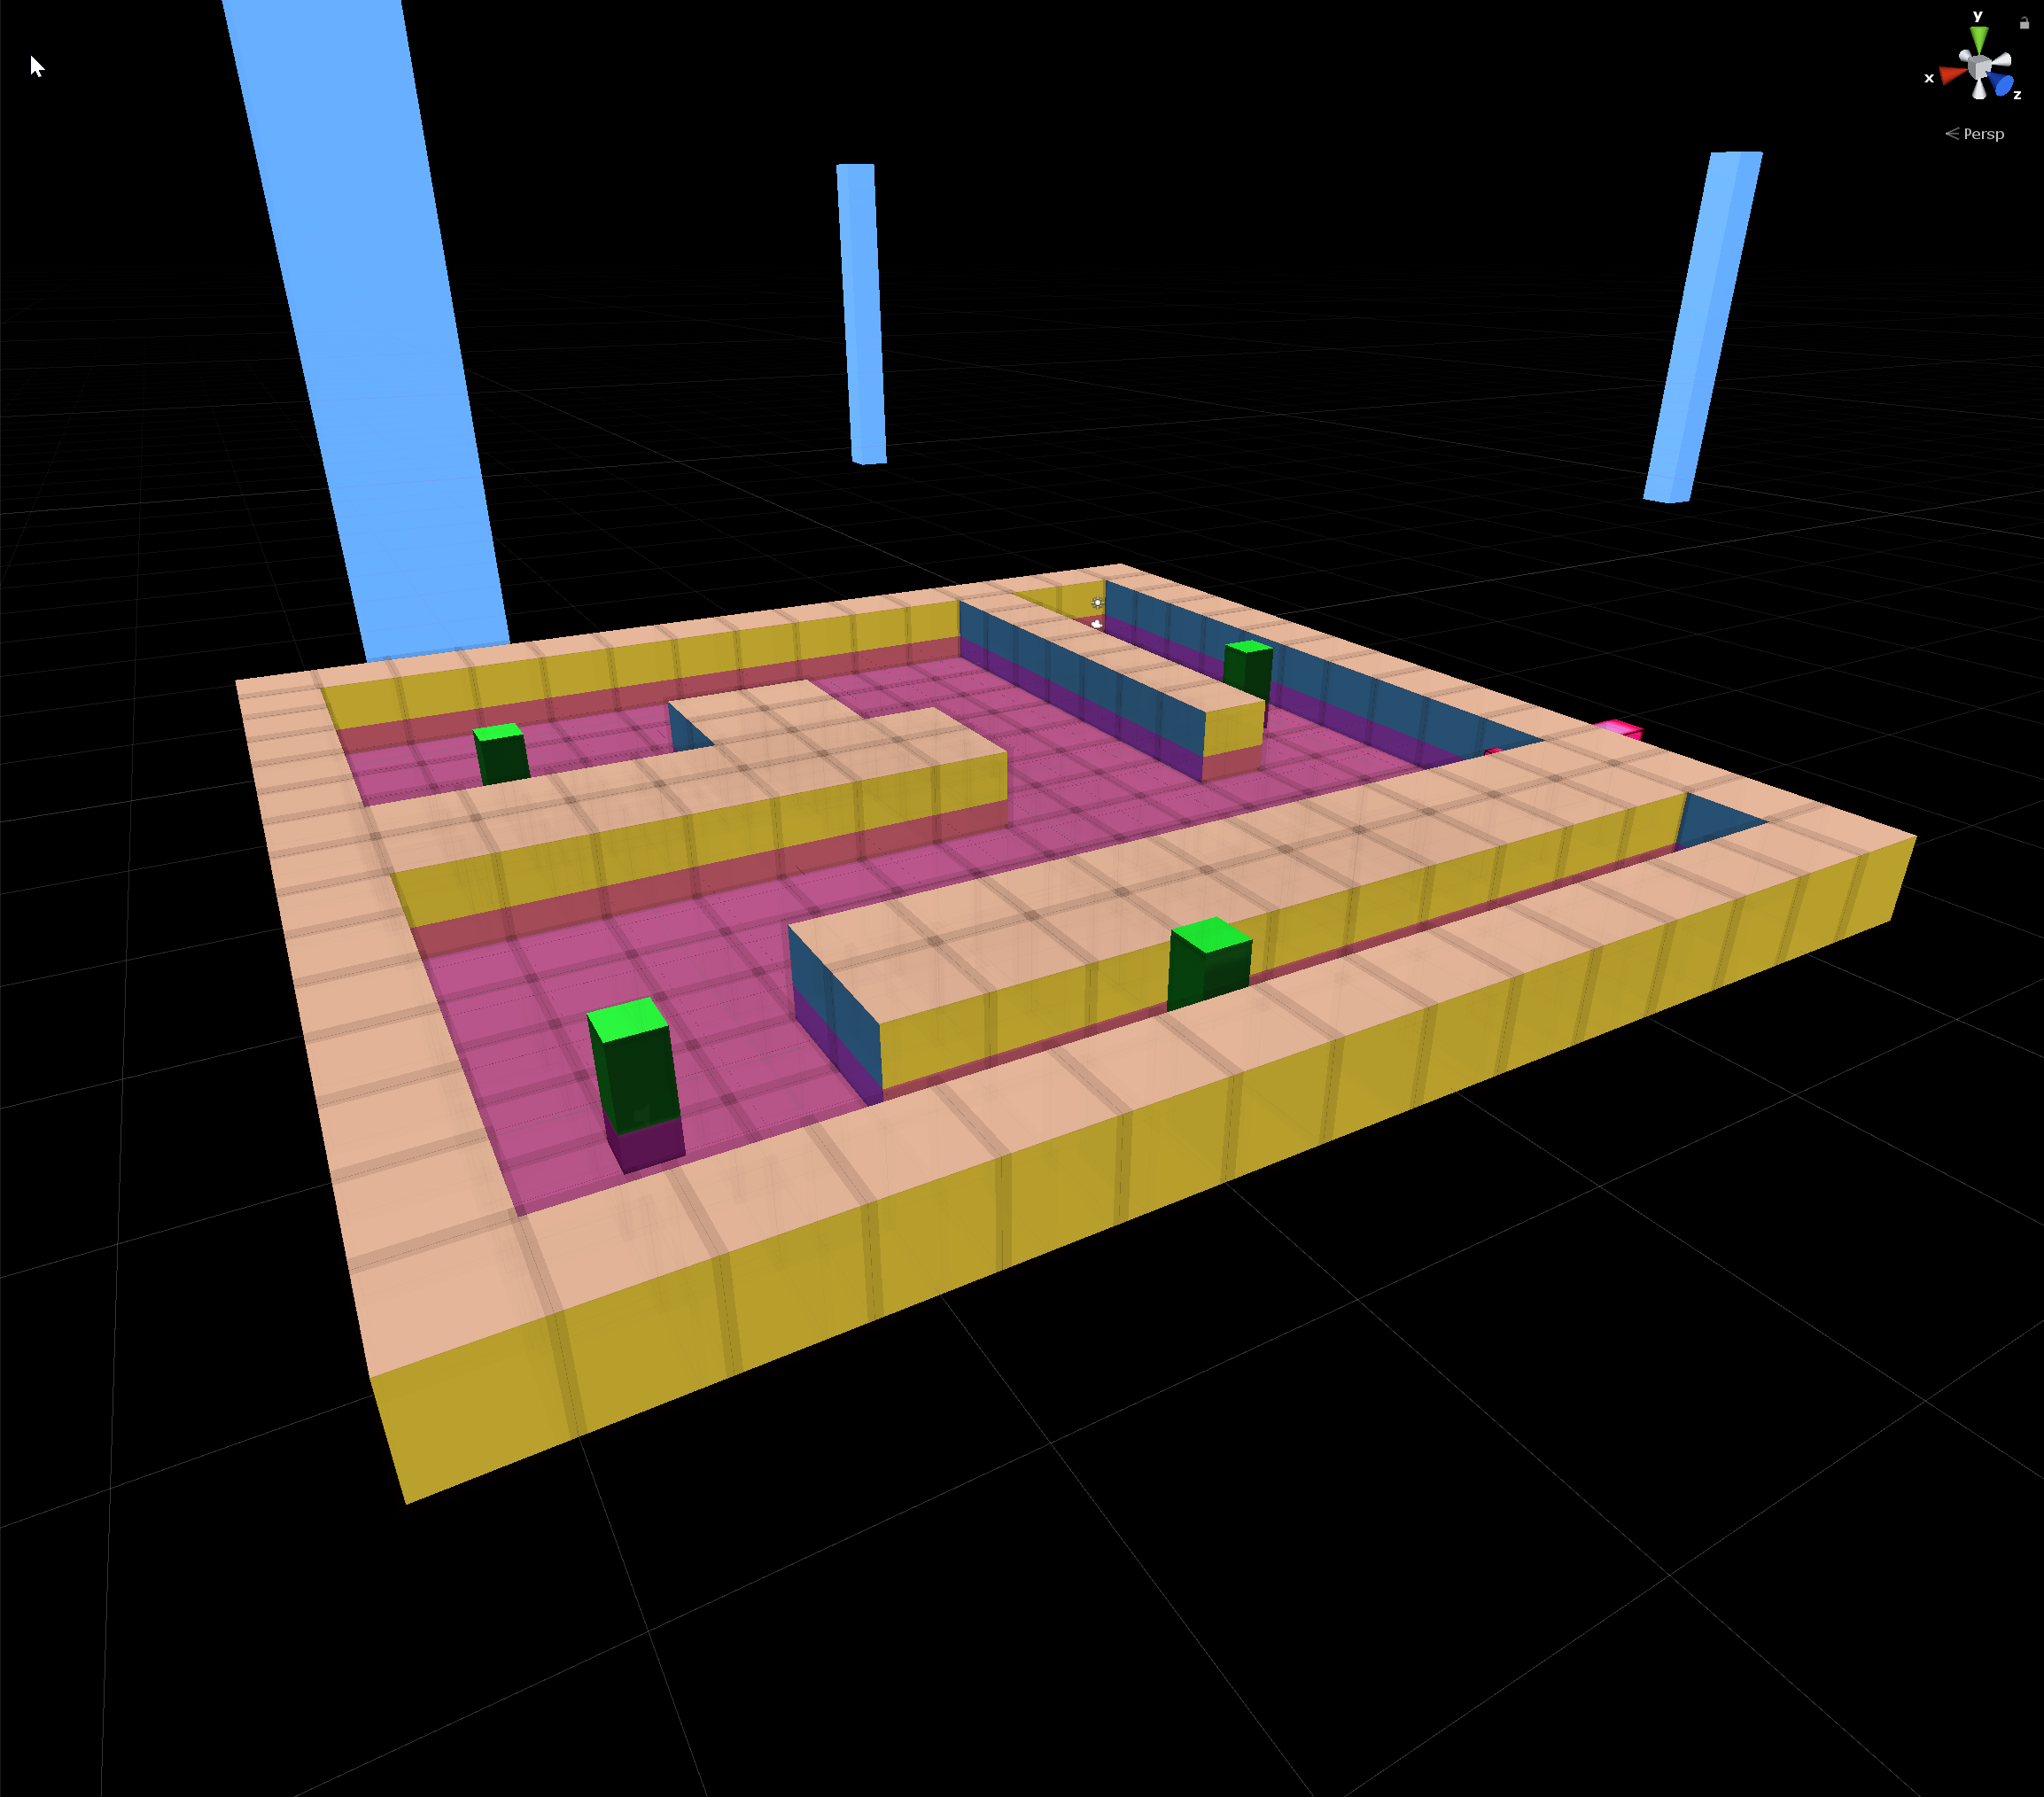
\includegraphics[width=\imgWidth]{images/neural_network_systems/NoKeyout.png} \\[\picVdist]
  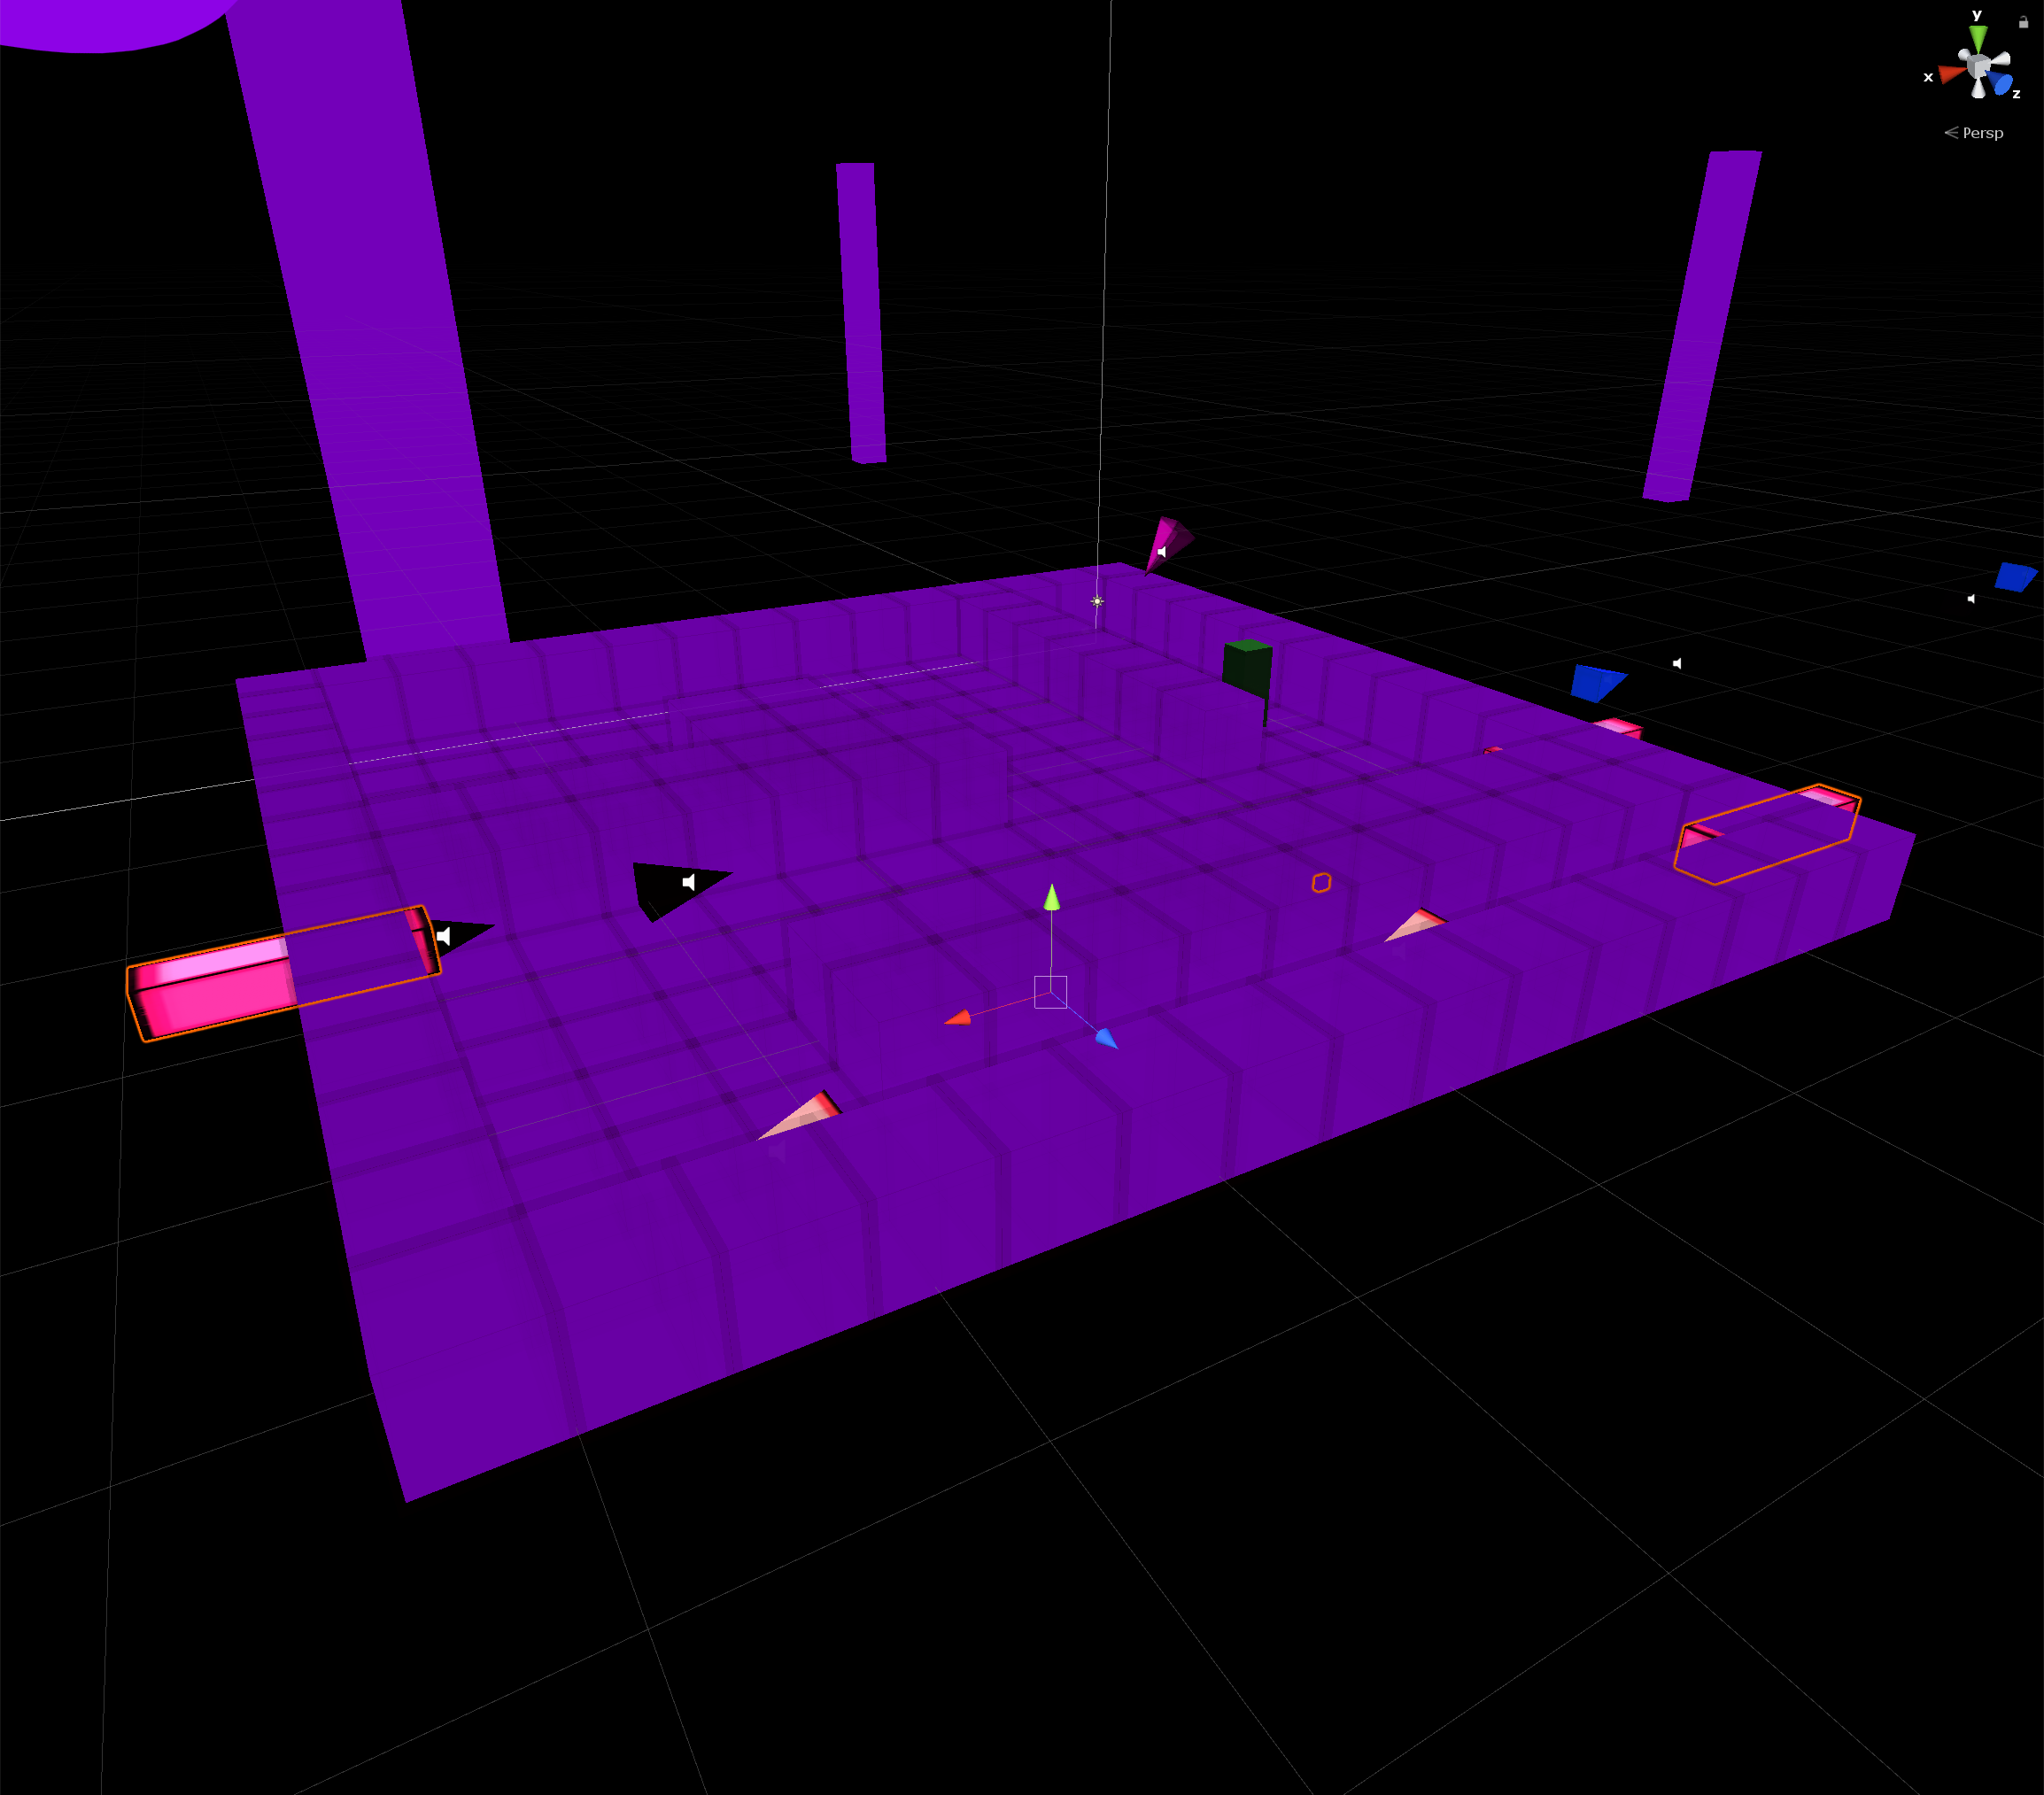
\includegraphics[width=\imgWidth]{images/neural_network_systems/WithKeyout.png}
  \caption{The keyout material is applied to everything that should not be visible.}
  \label{KeyoutEditor}
  \figsource{own graphic}
\end{figure}

\begin{figure}[p]
  \centering
  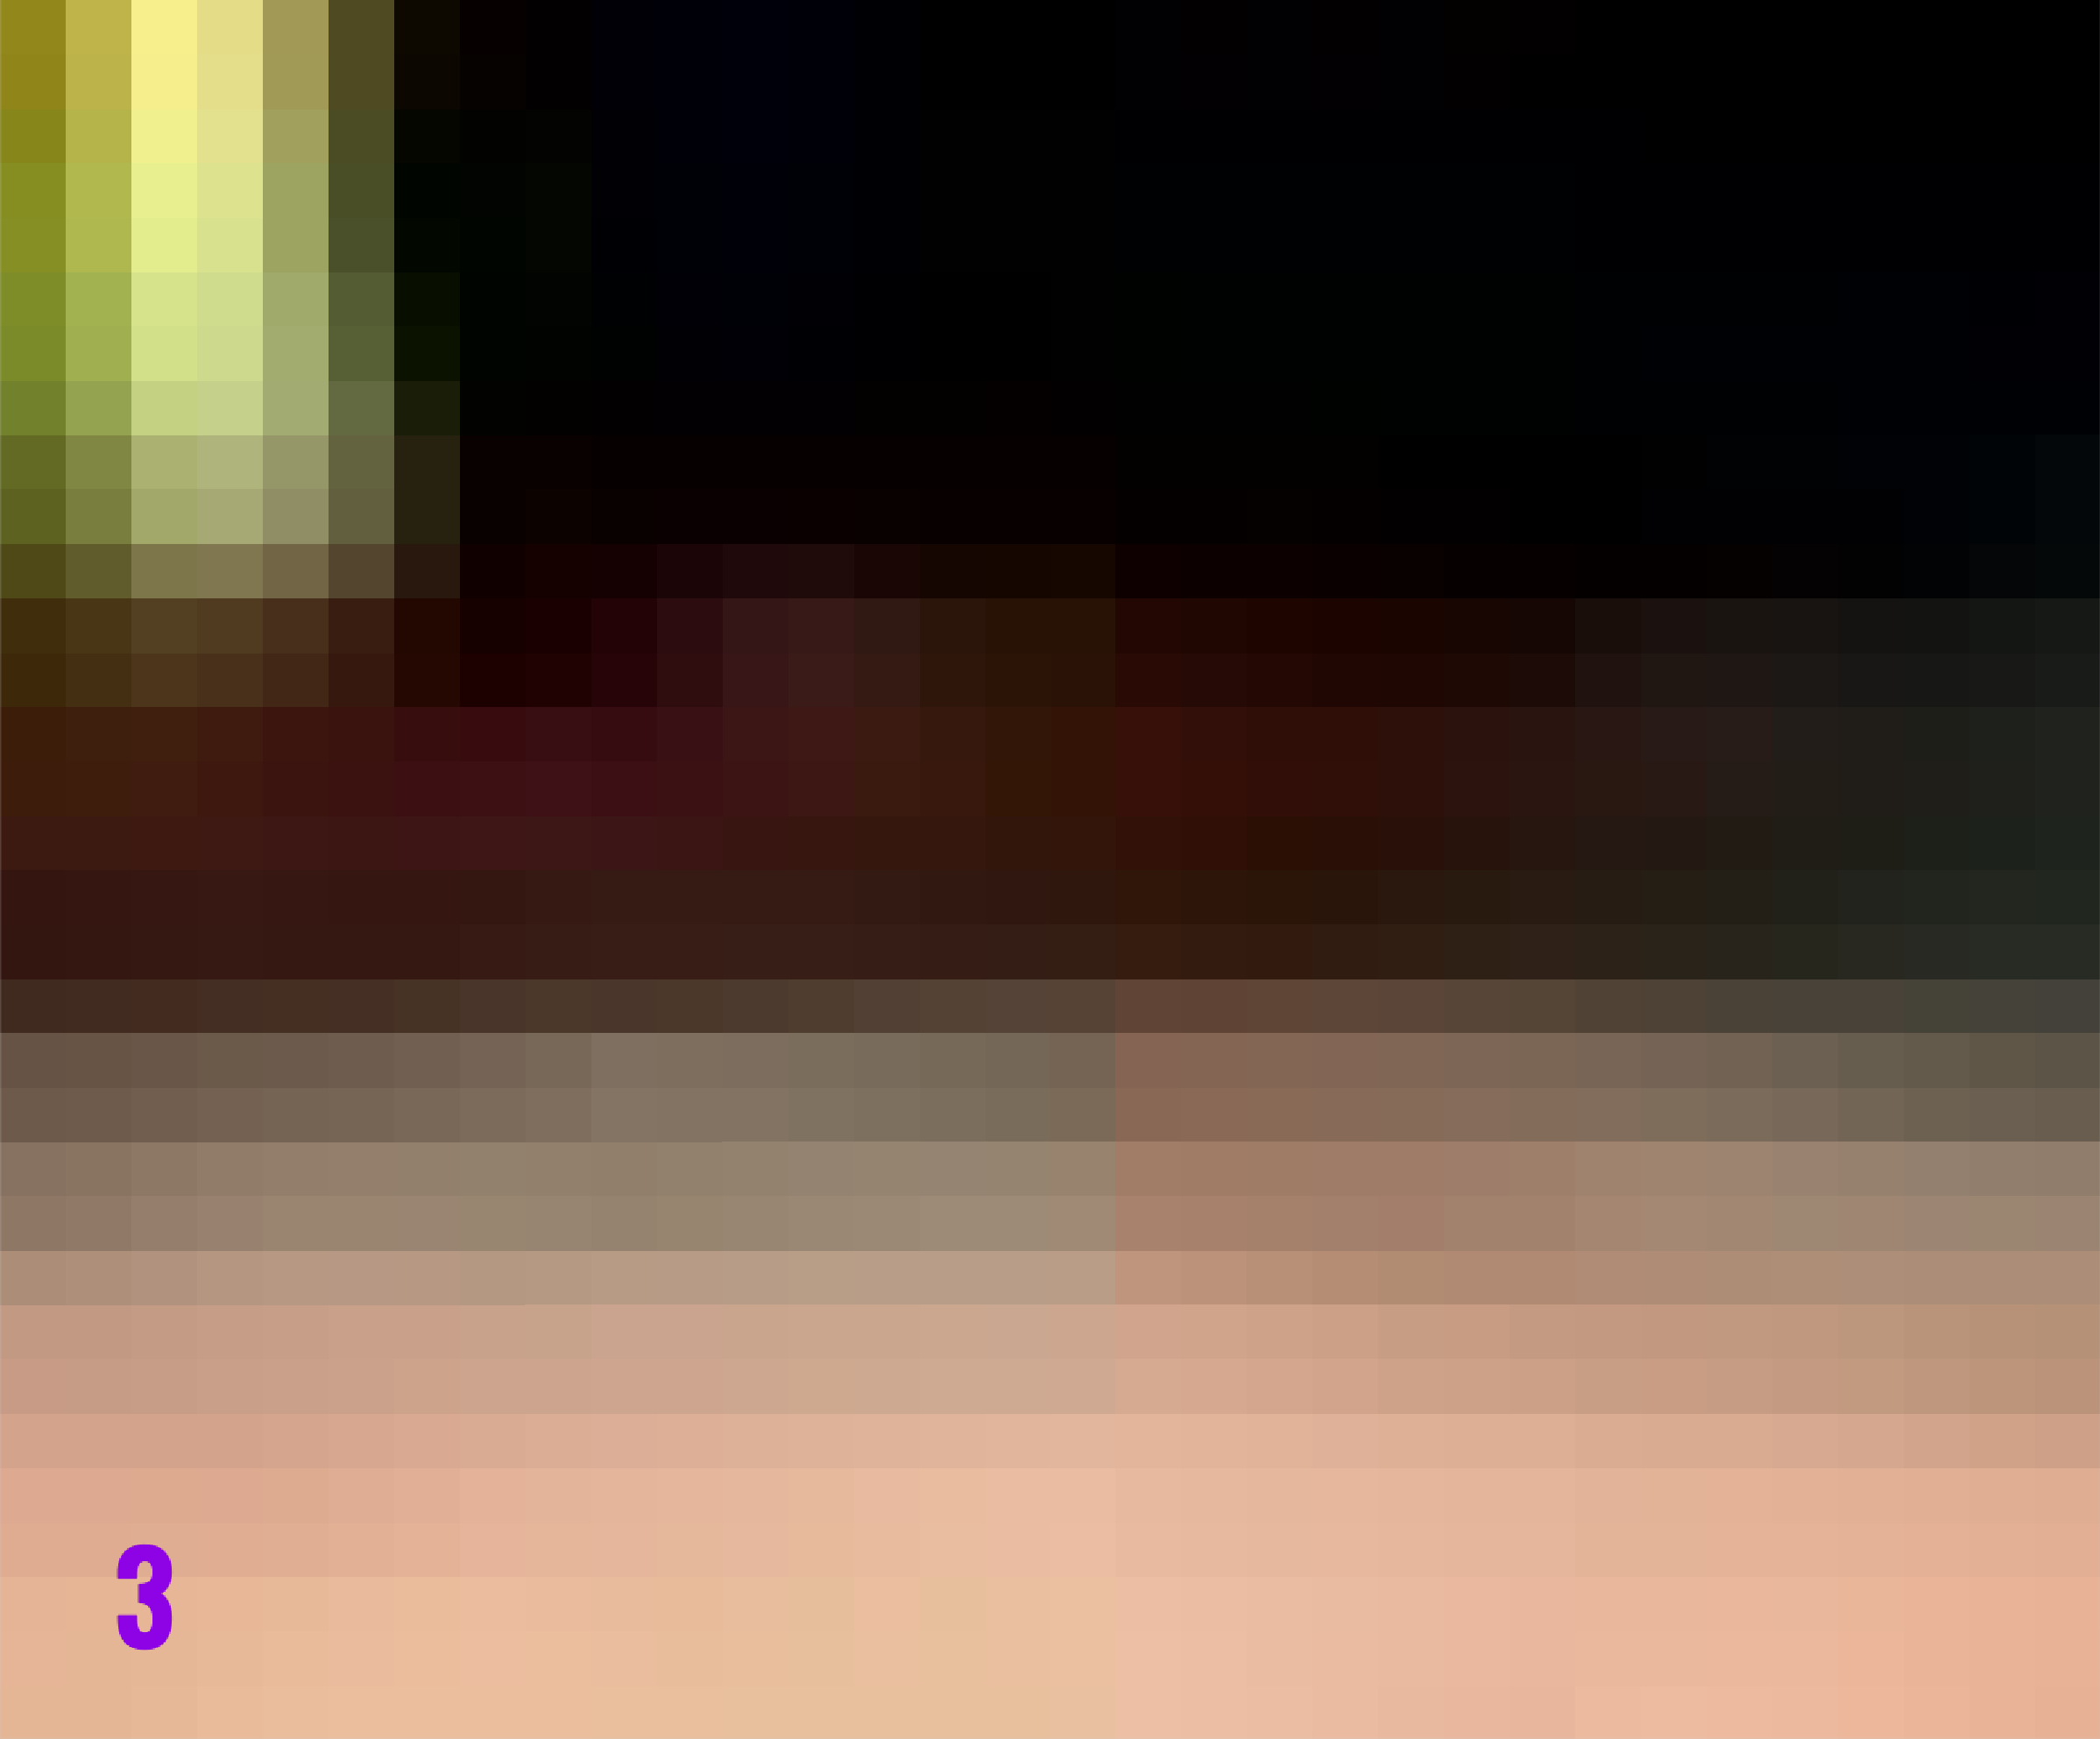
\includegraphics[width=\imgWidth]{images/neural_network_systems/NoOverlay.png} \\[\picVdist]
  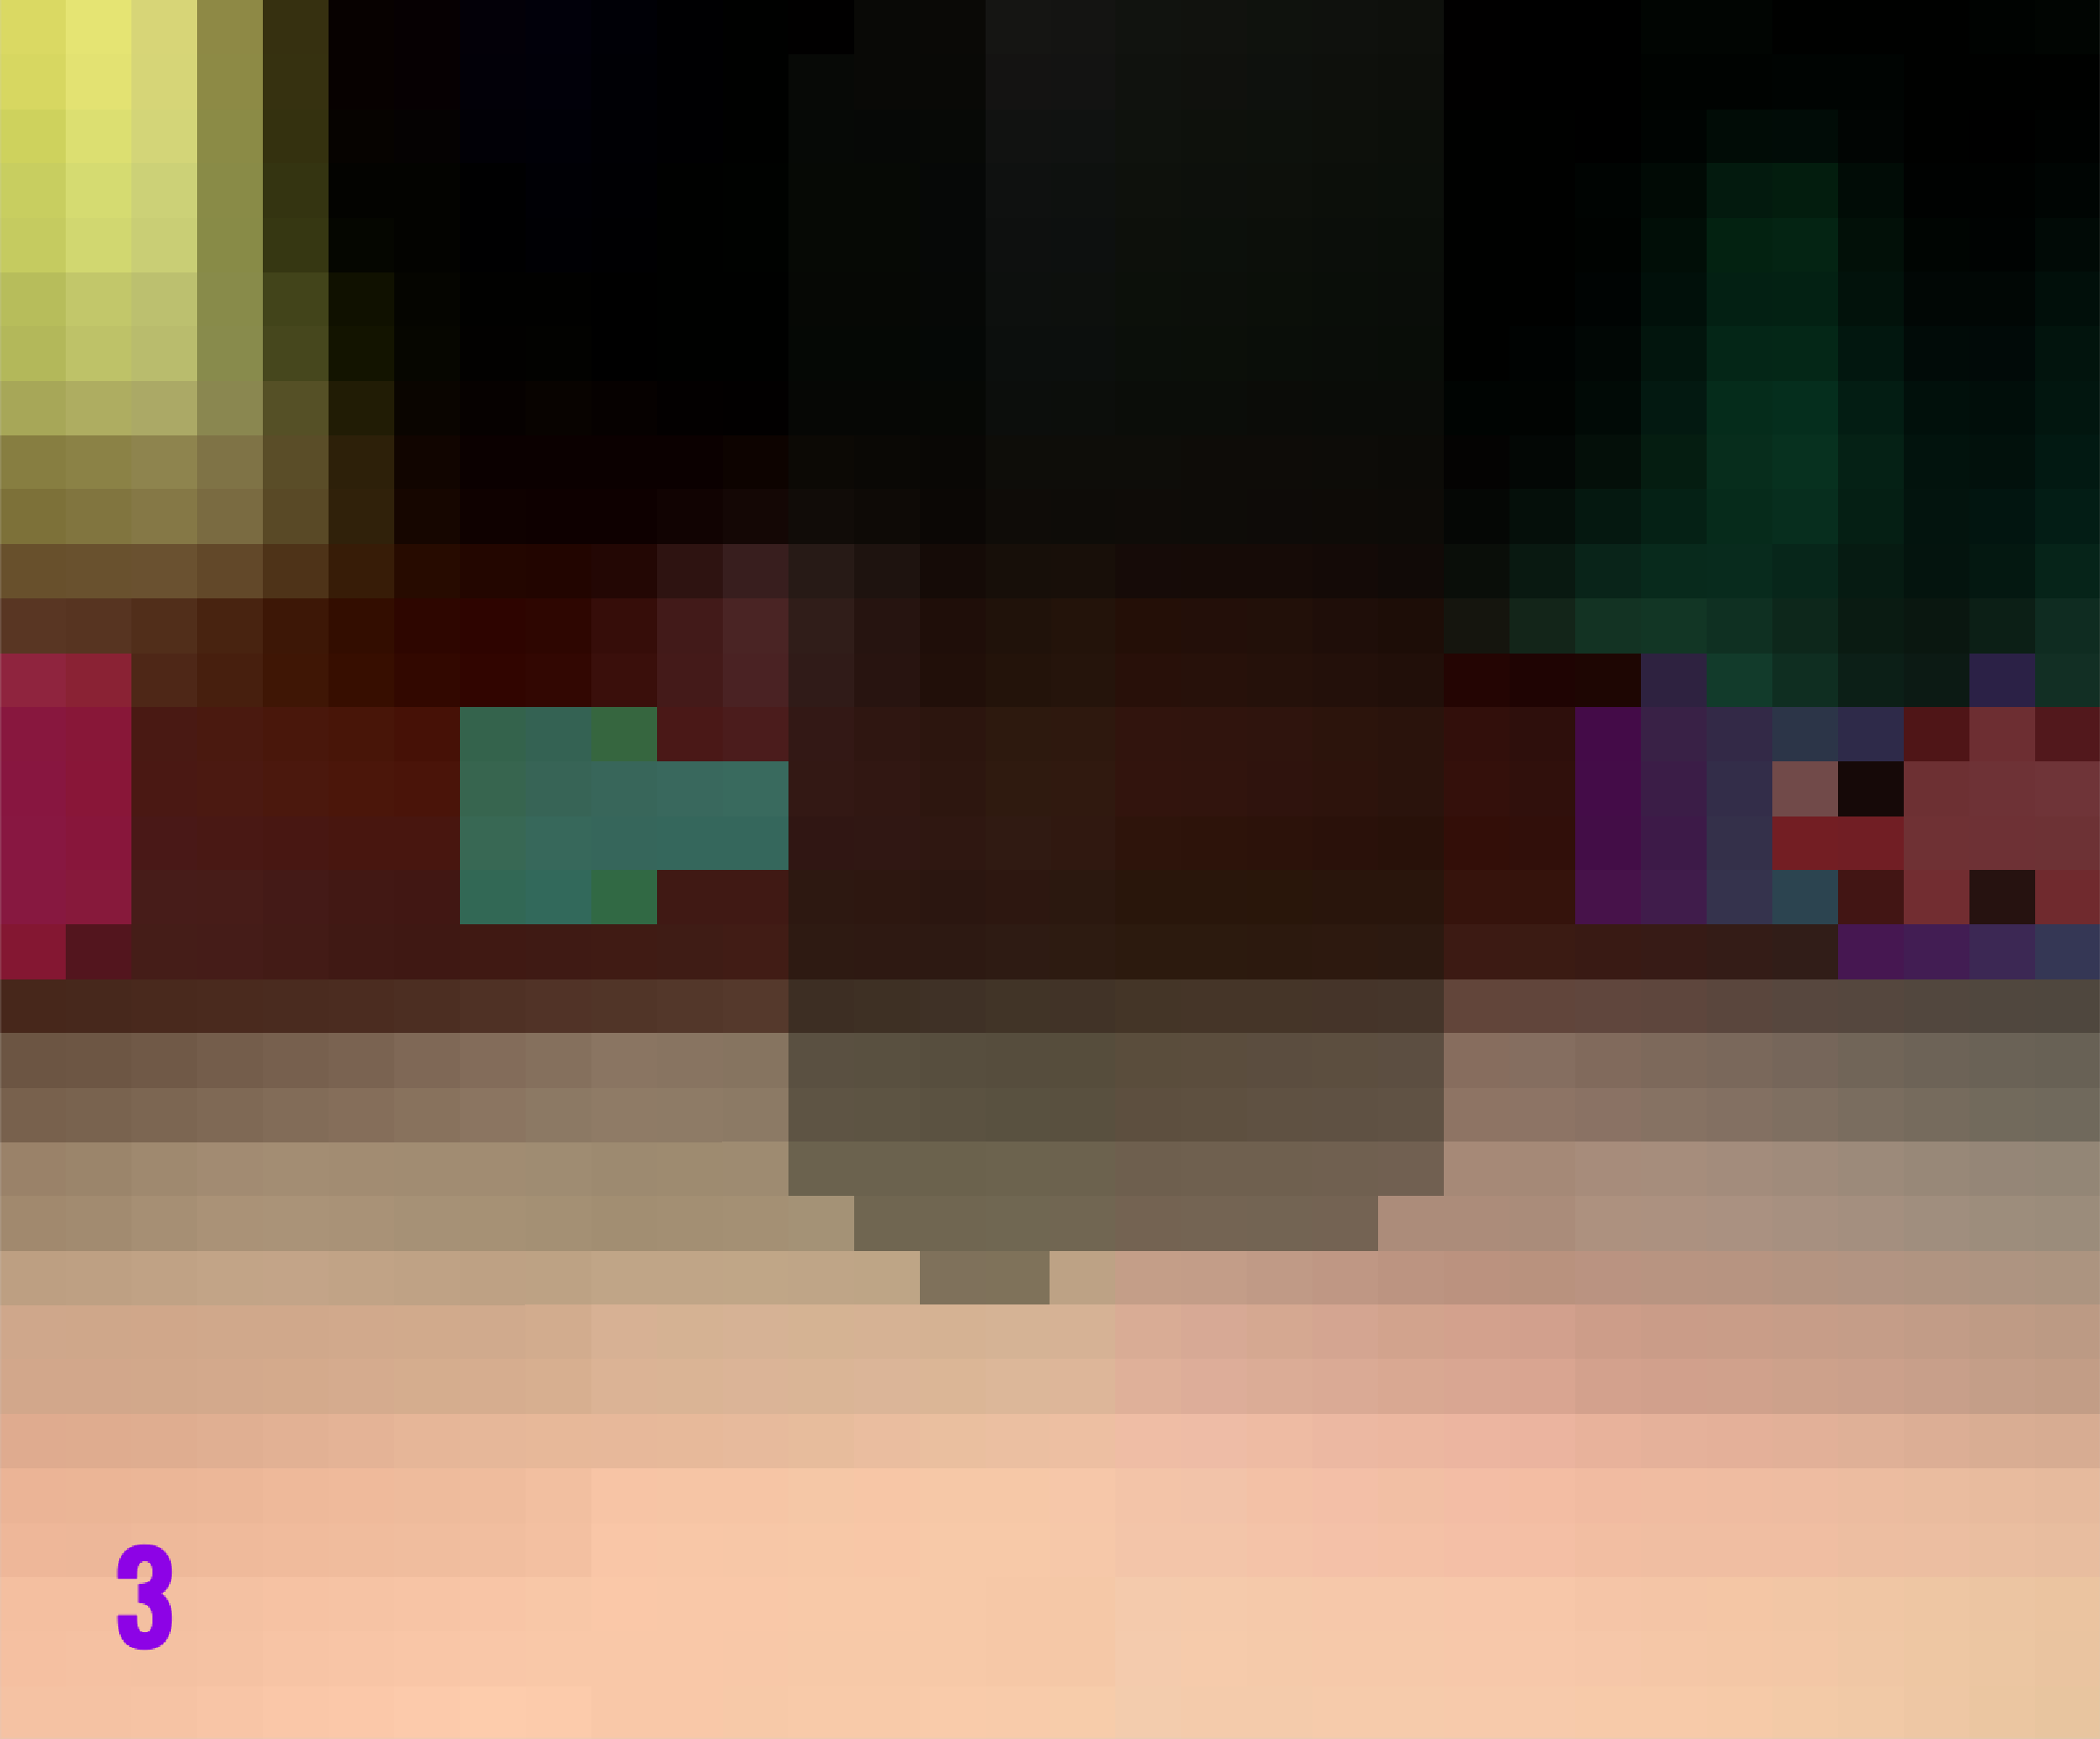
\includegraphics[width=\imgWidth]{images/neural_network_systems/WithOverlay.png}
  \caption{The network output is merged with the output of a Unity camera.}
  \label{RenderMerge}
  \figsource{own graphic}
\end{figure}


\subsection{Smoke ball rendering}\label{SmokeBallRendering}
The ability of smoke balls to reveal structural environment objects is created by having the smoke be additive particles. When the additive particles are rendered in front of objects that have the key-out color material, the color gets offset slightly so that it is no longer keyed out by the shader. The objects behind the smoke appear to the player as flat shaded surfaces with the key-out material.

Smoke balls can also be used to reveal the Invisible champer that is described in \cref{InvisibleChamper}. This works because the champer is keyed out by the same shader that keys out the environment. In unity the champer is not transparent but opaque. This means that if the champer is in front of smoke, he overwrites the smoke by getting his pixels in the image set to transparent. The player then sees a cutout in the smoke where only the network output is visible in the shape of the champer.
